\begin{frame}{\alert{Tâche} : Codage par transformée}
$$y = C(x) \in \mathbb{R}^Y | x \in \mathbb{R}^{X} \tilde{x} = C^{-1}(y), P_e(x) \simeq P_e(\tilde{x})$$
\begin{itemize}
\item $C$ : Quantification adaptative d'un équivalent de la Transformée de Fourier à Court Terme (TFCT)
\item $P_e$ : Modélisation de la sensibilité aux déformations de la membrane basilaire\footfullcitenomarkleft{Zwicker}{}{}{}
\end{itemize}
Gain : $Y<<X$
Validation : écoute
\end{frame}

\begin{frame}{Transformée de Fourier à Court Terme (TFCT)}
$$ X[m, t] = \sum_{n = - \infty}^{\infty} x[n] w[n-t] \mathrm{e}^{\frac{-2 \mathrm{j}  \pi m n}{N}} $$
\end{frame}

\begin{frame}{Spectrogramme : $|X[m, t]|$}
\begin{center}
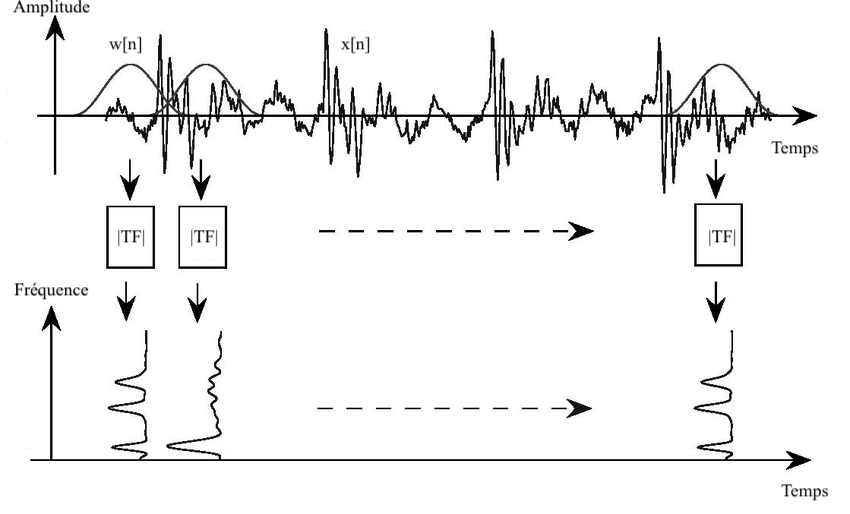
\includegraphics[width=.9\columnwidth]{figures/tfct} \\
\end{center}
\end{frame}

\begin{frame}{Typologie des évènements sonores}
\begin{description}
  \item[parole] : sons voisés <a>, <o> / sons plosifs <pe>, <qe>;
  \item[communication animale] : hululement de chouettes / clics de localisation de chauve souris;
  \item[musique] : chant lyrique / percussions;
  \item[mécanique] : ventilation / marteau piqueur;
  \item[environnementaux] : vent faisant siffler des câbles / gouttes de pluie tombant sporadiquement.
\end{description}
\end{frame}

\begin{frame}{Compromis temps/fréquence}
\begin{center}
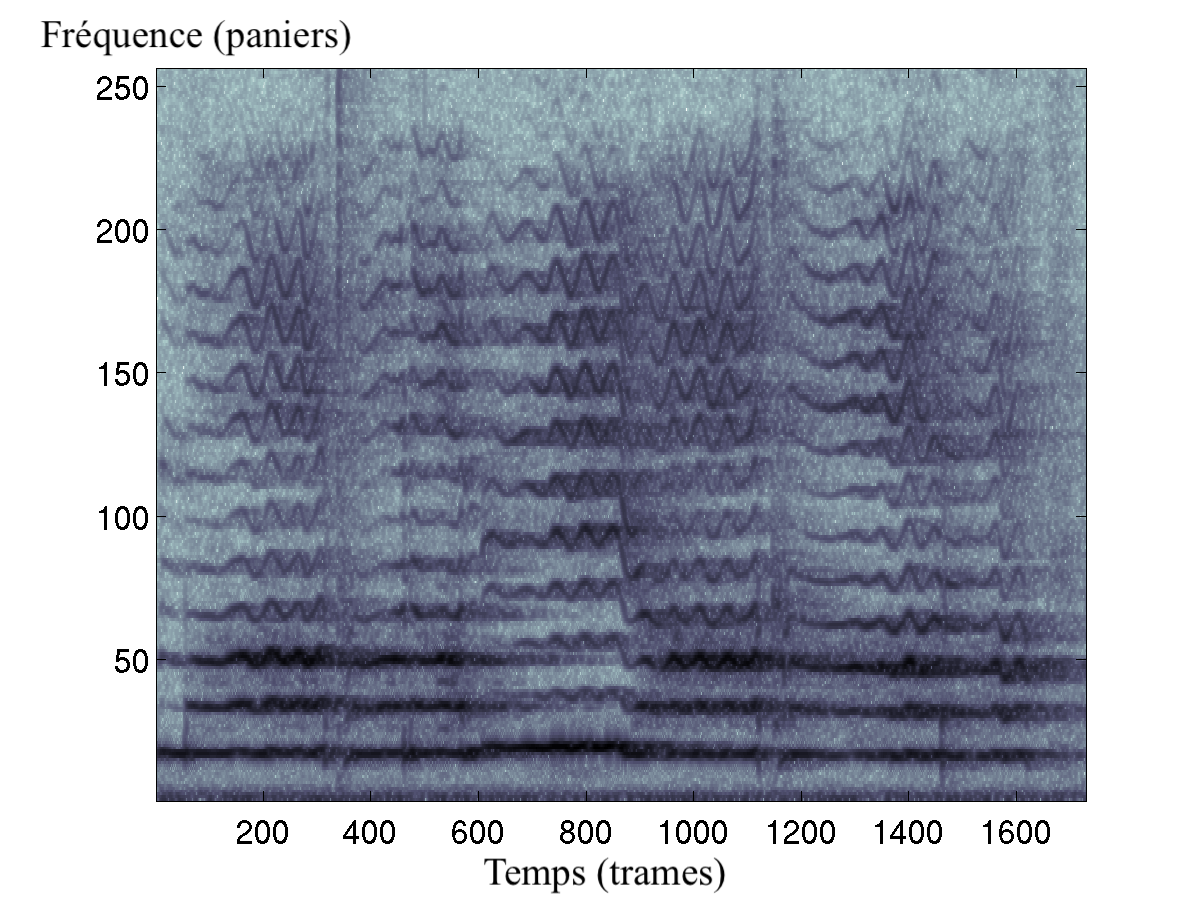
\includegraphics[width=.7\columnwidth]{figures/soloSpec} 
\end{center}
	$\hookrightarrow{}$ mitiger cette contrainte imposée par l'approche court-terme par l'utilisation d'\alert{\textit{a priori}} sur les sources d'intérêt.
\end{frame}

\begin{frame}{Analyse de Scènes Auditives Computationelle (CASA)}
L'ASA\footfullcitenomarkleft{bregman1994auditory} étudie l'ensemble de traitements perceptifs permettant
\begin{itemize}
\item d'isoler les informations émanant d'\structure{entités} sonores distinctes,
\item de les organiser en un tout cohérent.
\item à l'aide de processus \structure{\og primitifs \fg} et \structure{\og séquentiels \fg}.
\end{itemize}
L'Analyse de Scènes Auditives Computationnelle (CASA)\footfullcitenomarkleft{wang2016casa} se propose de mettre en \oe~euvre ces critères pour inférer une organisation perceptuellement valide de la scène sonore.
\end{frame}

\begin{frame}{Processus ASA \og primitifs \fg}
\begin{description}
\item[\alert<2>{continuité}] : les propriétés d'un son isolé tendent à se modifier lentement et de façon continue
\item[harmonicité] : lorsqu'un corps sonore vibre à une période répétée, ses vibrations donnent naissance à un motif acoustique dont les fréquences des composants sont des multiples d'une même fréquence fondamentale;
\item[...]
\end{description}
\end{frame}

\begin{frame}{Modèle sinusoïdal à long terme}
\only<1>{
$$
x[n]=\sum_{l=1}^{L} a_{l}[n] \sin \left(\frac{2 \pi}{F_{s}} f_{l}[n] \cdot n + \Phi_k \right)
$$
$a_{l}[n]$ et $f_{l}[n]$ sont des signaux contrôlant respectivement l'amplitude et la phase des $L$ oscillateurs composant le modèle.
}
\only<2>{mettre le son et la figure} %http://webpages.mcgill.ca/staff/Group2/abregm1/web/snd/Track24.mp3
\end{frame}

\begin{frame}{Traitement}
\begin{center}
\begin{tikzpicture}[
nonterminal/.append style={join=by ->},
tip/.style={->,shorten >=1pt},every join/.style={rounded corners},
terminal/.style={
% The shape:
rectangle,minimum size=6mm,rounded corners=1mm,
% The rest
very thick,draw=black!50,
top color=white,bottom color=black!10,
font=\ttfamily},
point/.style={circle,fill=black,minimum size=2pt},
%every node/.style=draw,
line/.style ={draw, thick, -latex',shorten
  >=2pt}]
  
  \matrix [column sep=10mm,row sep=5mm]
{
\node (i1) {}; \\
\node [terminal] (i2) {tfct}; \\
\node [terminal] (i3) {sélection de pics}; \\
\node [terminal] (i4) {suivi de partiel}; \\
\node  (i5) {}; \\
};

\begin{scope}[every path/.style=line]
  \path (i1) -- node [right] {signal} (i2);
  \path (i2) -- node [right] {spectrogramme} (i3);
  \path (i3) -- node [right] {atomes } (i4);
  \path (i4) -- node [right] {partiels} (i5);
\end{scope}
\end{tikzpicture}
\end{center}
\end{frame}

\begin{frame}{Atomes temps/fréquences}
\begin{center}
 \only<1>{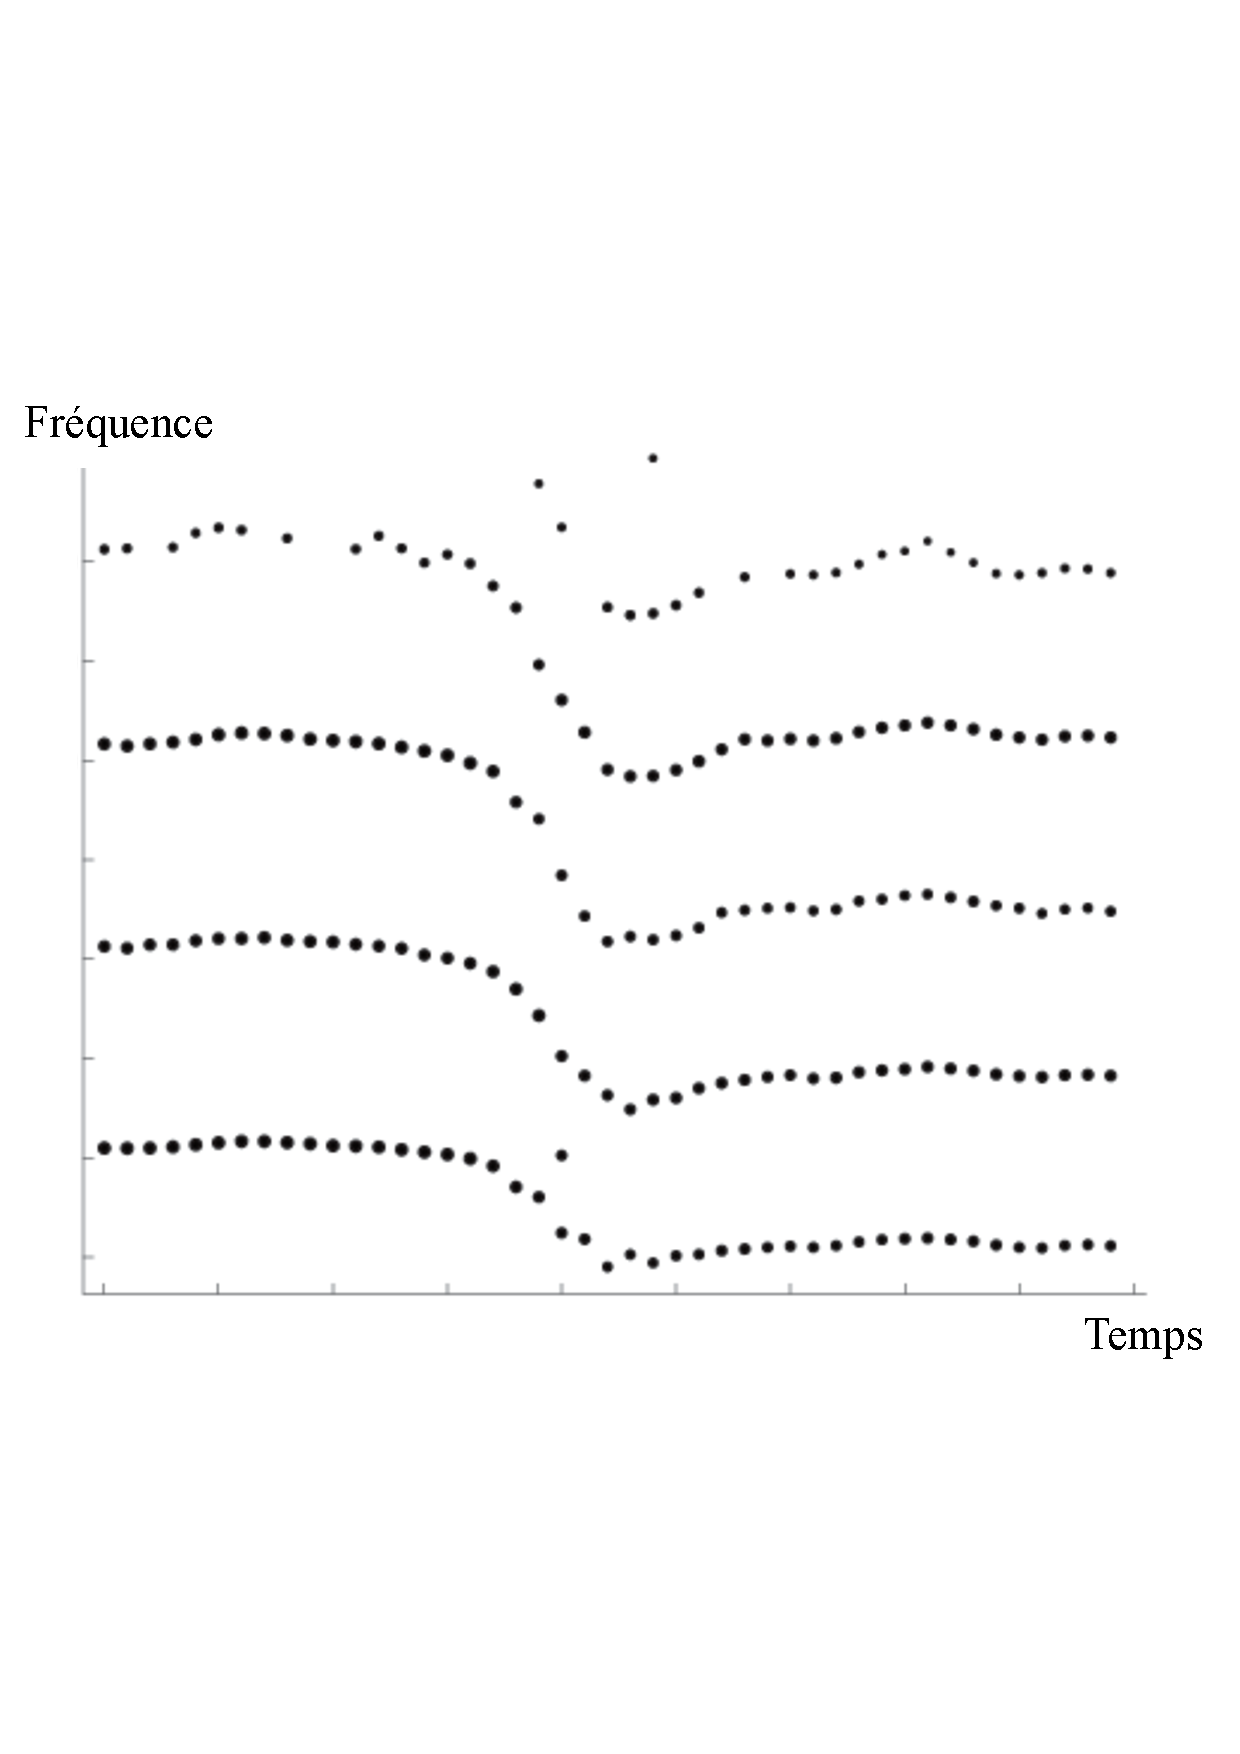
\includegraphics[width=.7\textwidth]{voice_1024_512xp} \\
 Taille de fenêtre : \structure{23} ms, pas d'avancement 10 ms.}
 \only<2>{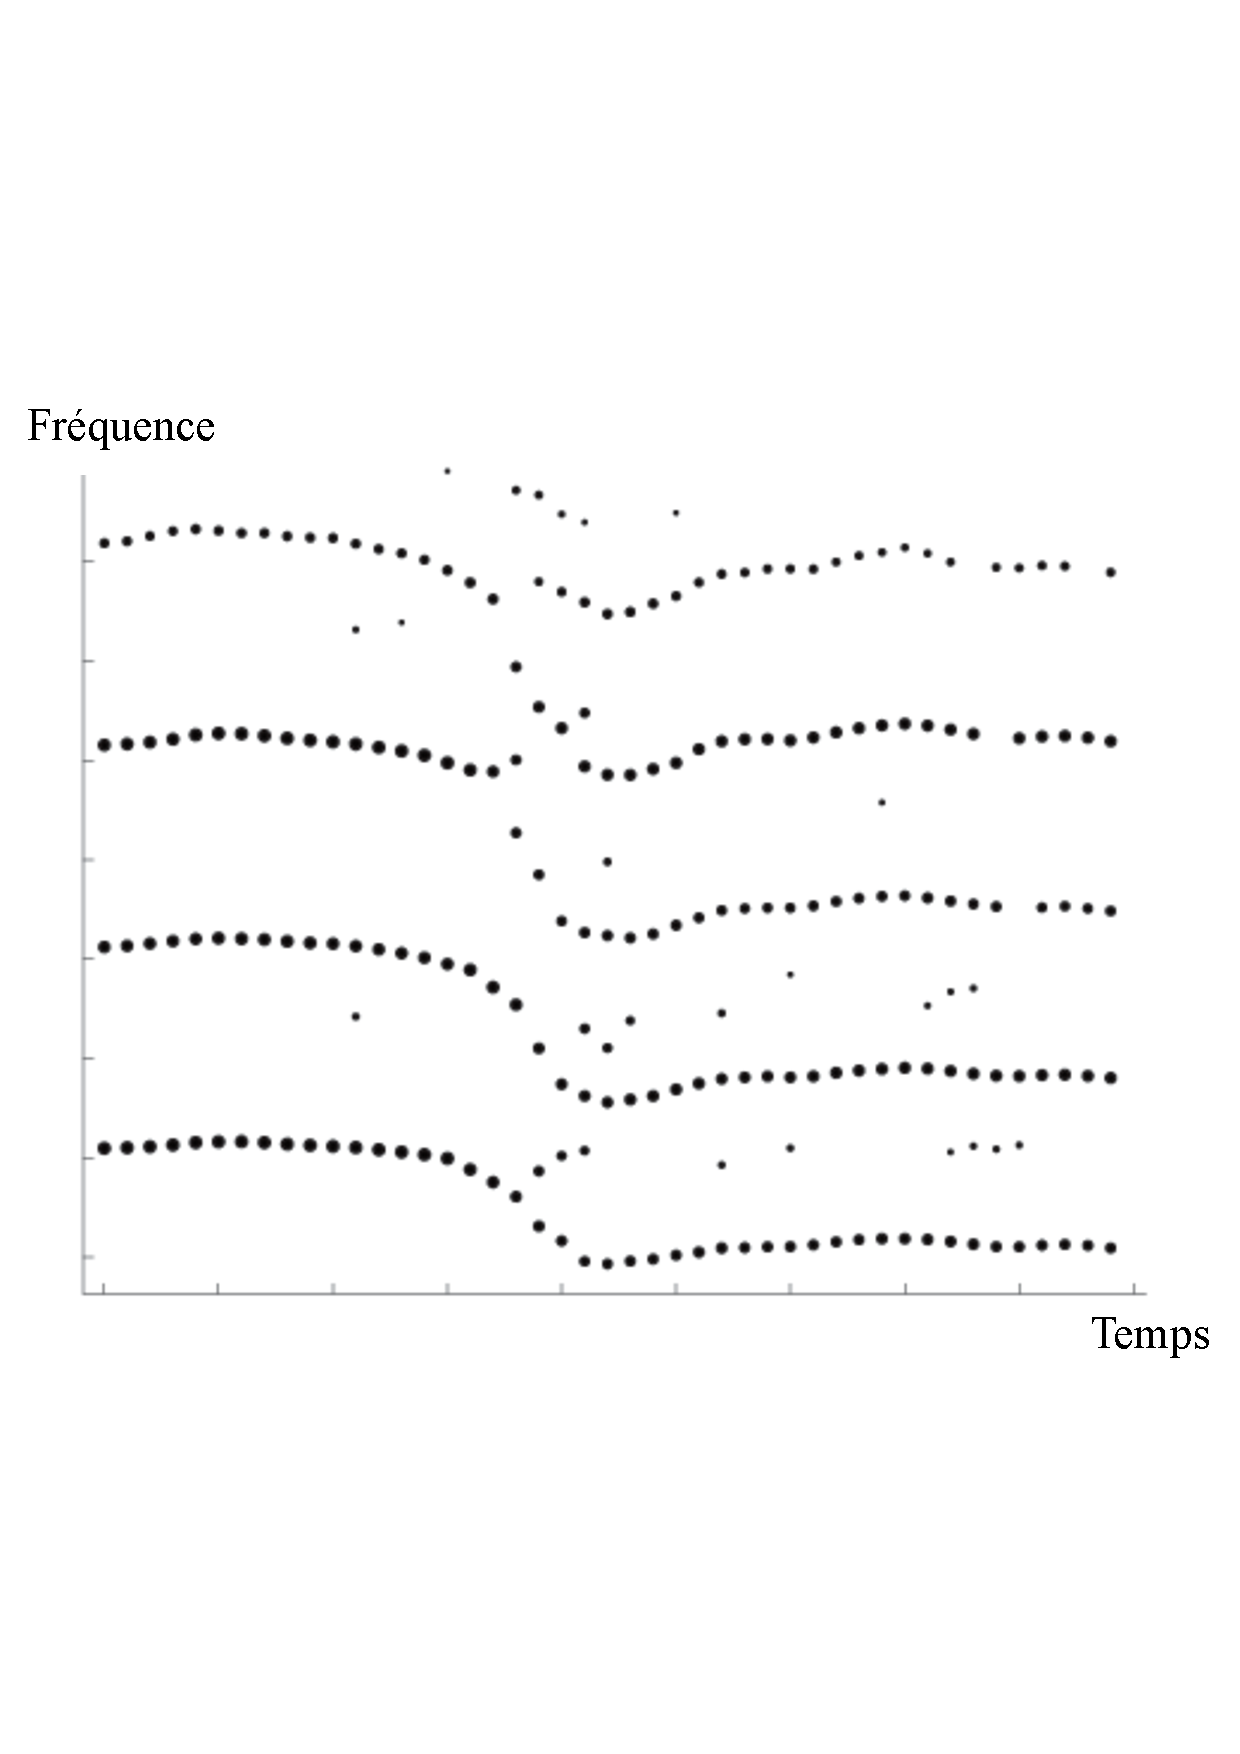
\includegraphics[width=.7\textwidth]{voice_2048_512xp} \\
 Taille de fenêtre : \structure{46} ms, pas d'avancement 10 ms.}
 \only<3>{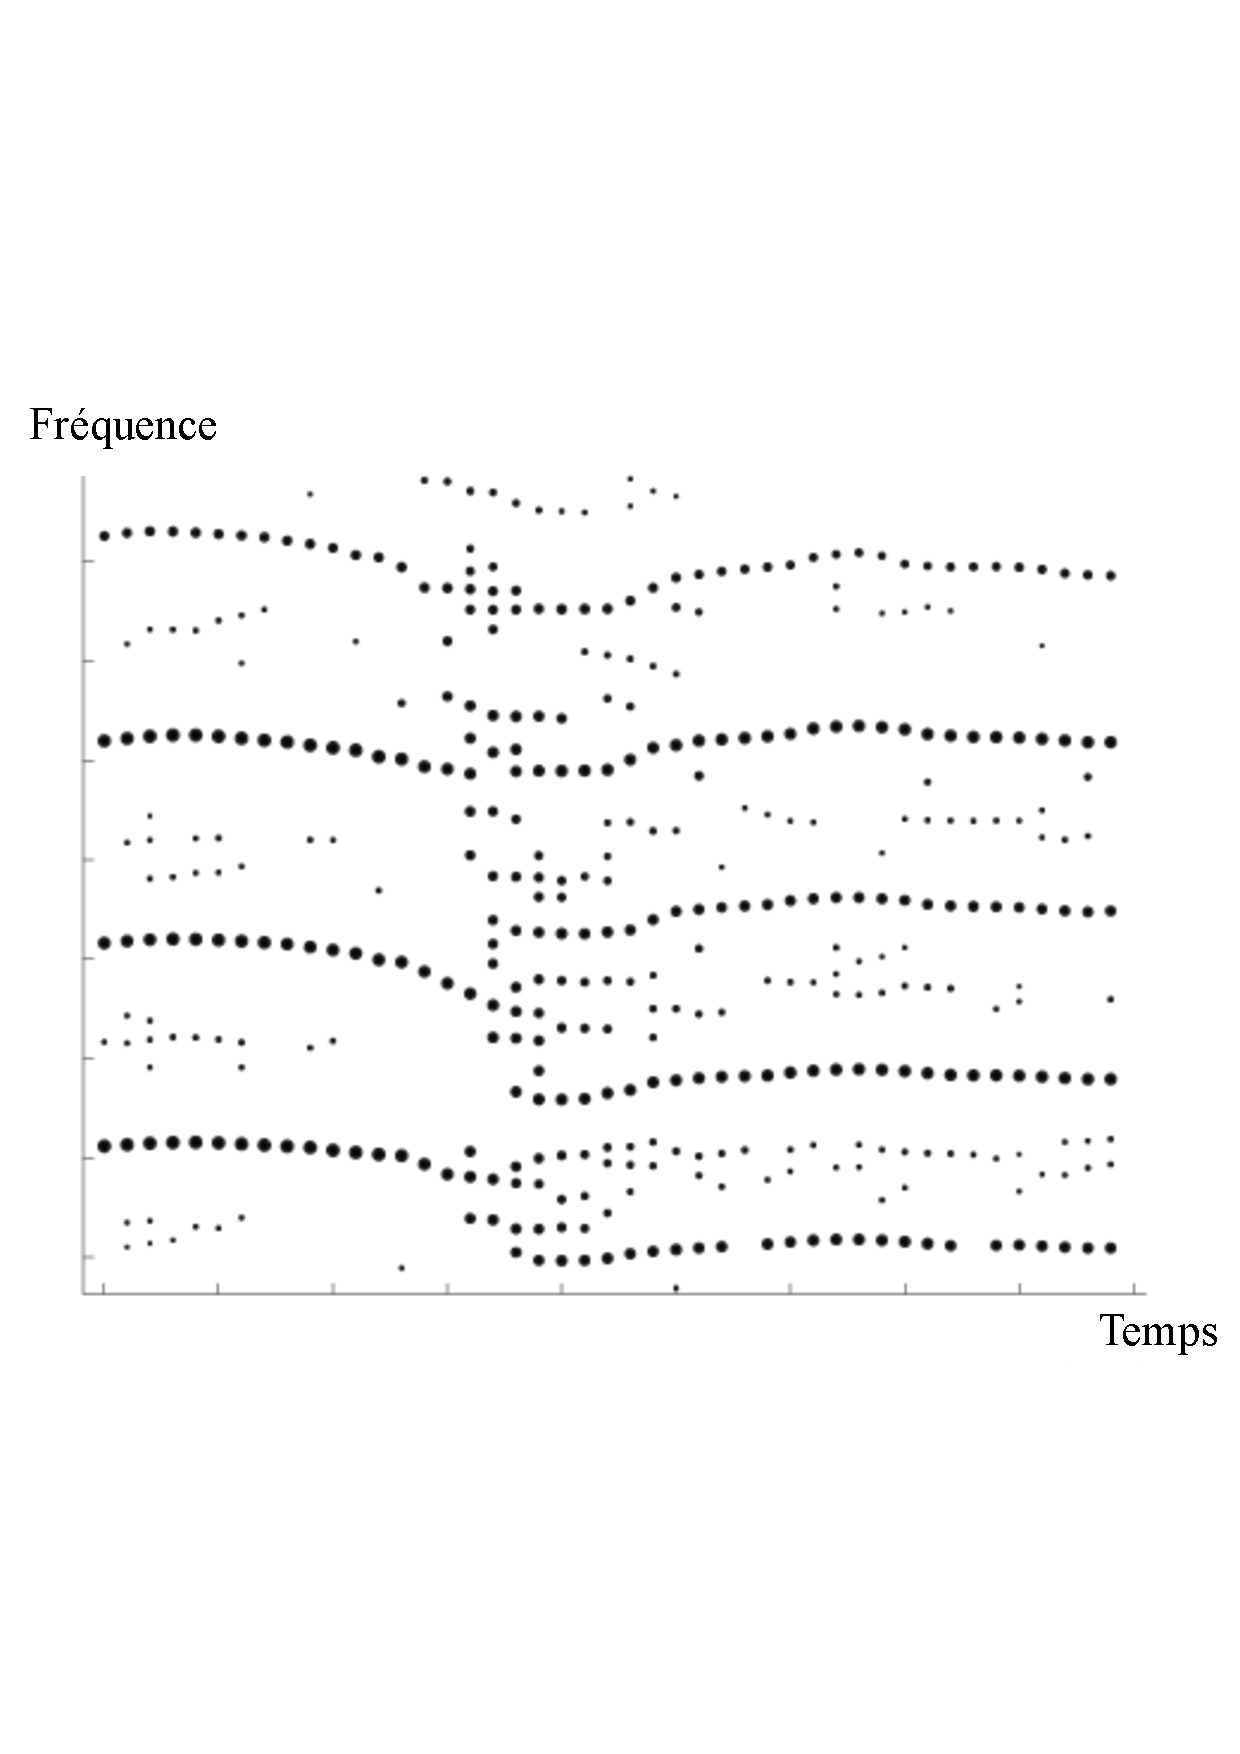
\includegraphics[width=.7\textwidth]{voice_4096_512xp} \\
 Taille de fenêtre : \structure{92} ms, pas d'avancement 10 ms.}
\end{center}
\end{frame}

\begin{frame}{Algorithme de suivi amélioré\footfullcitenomarkleft{lagrangeTaslp06}}
\begin{center}
  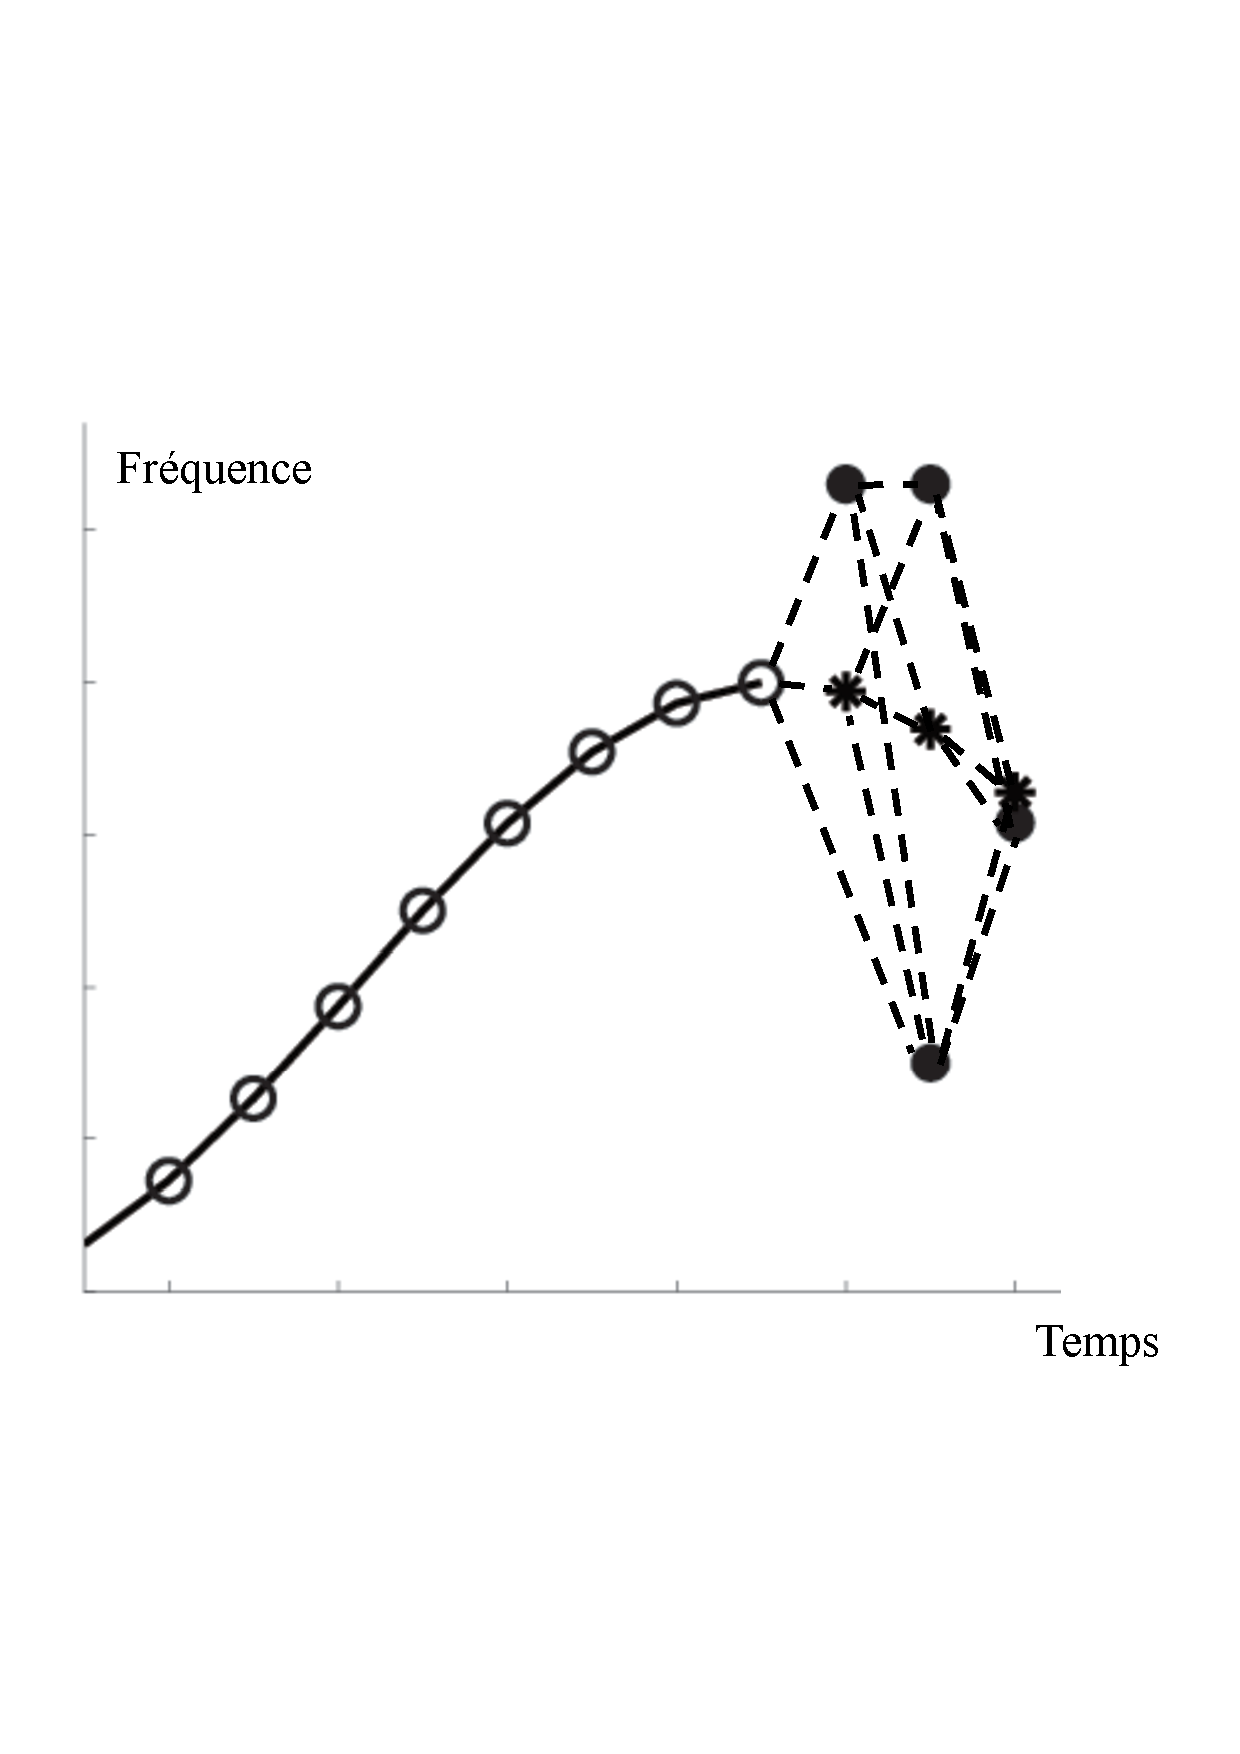
\includegraphics[width=.4\textwidth]{trackingxp2xp2}
\end{center}
  \begin{enumerate}
      \item Prédiction auto-régressive de l'évolution des paramètres de fréquence et d'amplitude
      \item Sélection des continuations engendrant le moins de hautes fréquences
  \end{enumerate}
\end{frame}

\begin{frame}{Processus ASA \og primitifs \fg}
\begin{description}
\item[\alert{continuité}] : les propriétés d'un son isolé tendent à se modifier lentement et de façon continue
\item[\alert{harmonicité}] : lorsqu'un corps sonore vibre à une période répétée, ses vibrations donnent naissance à un motif acoustique dont les fréquences des composants sont des multiples d'une même fréquence fondamentale;
\item[...]
\end{description}
\end{frame}
 
\begin{frame}{Algorithme par coupures normalisées de graphes}
\begin{center}
 \only<1>{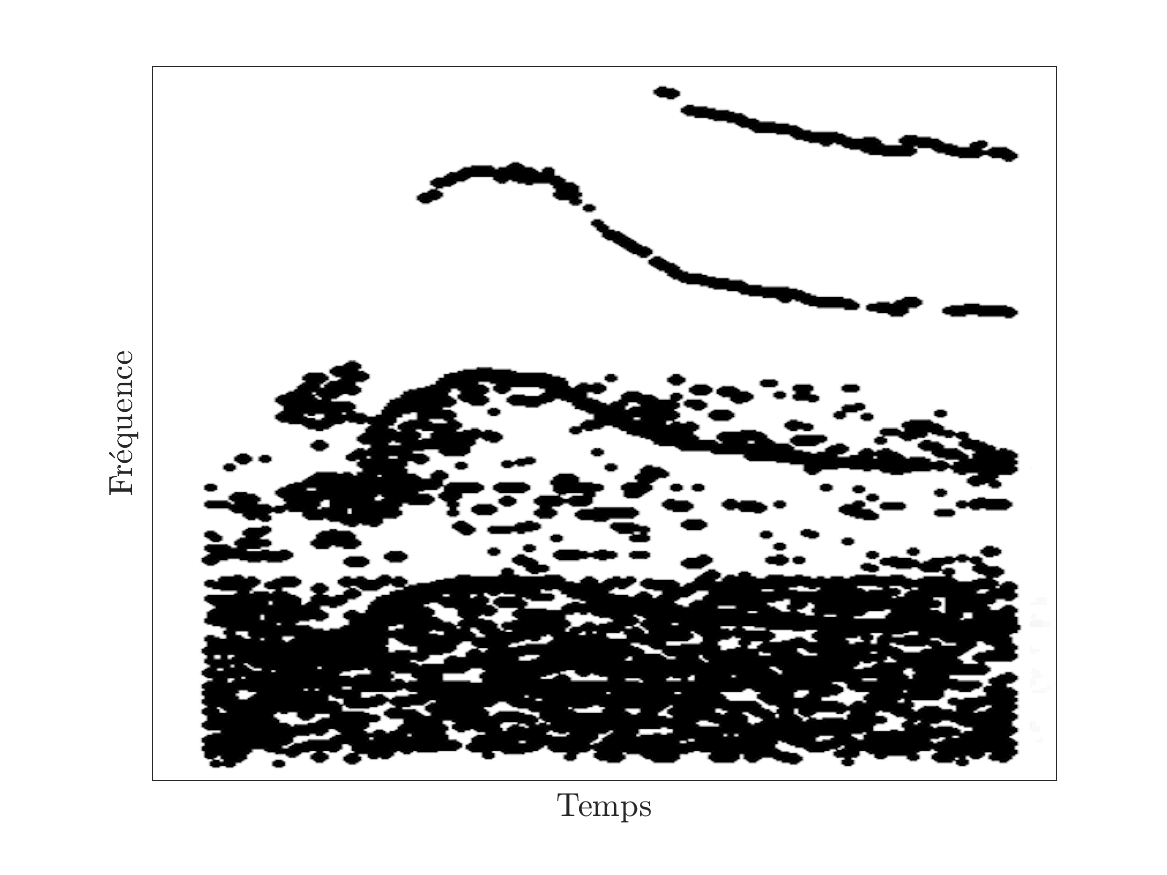
\includegraphics[width=.7\textwidth]{orcaSin}}
 \only<2>{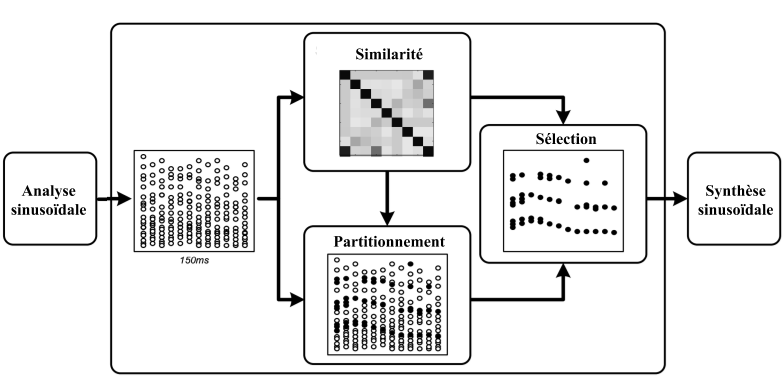
\includegraphics[width=.8\textwidth]{figures/ncutDiagramFr} \footfullcitenomarkleft{shi2000normalized}}
 \only<3>{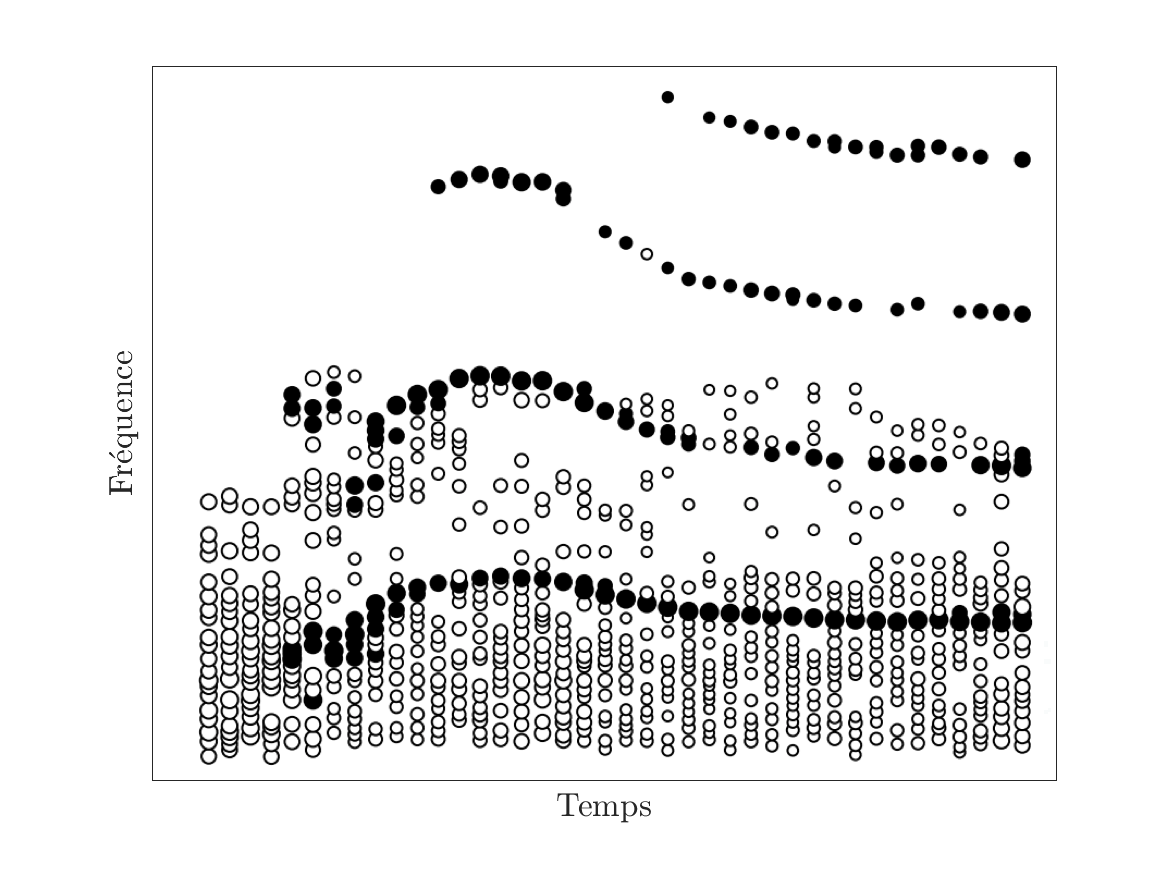
\includegraphics[width=.7\textwidth]{orcaSep}  \footfullcitenomarkleft{lagrangeTaslp08}}
\end{center}
\end{frame}



\begin{frame}{Processus ASA \og séquentiels \fg}
\begin{description}
\item[proximité] : des éléments proches les uns des autres sur le plan temps/fréquence ont tendance à être groupés ensemble
\item[similarité] : des éléments qui se ressemblent ont tendance à être groupés ensemble (timbre). 
\item[...]
\end{description}
\end{frame}

\begin{frame}{Regroupement hiérarchique alterné (ANR JCJC Houle)}
\footfullcitenomarkleft{rossignol2018efficient}
\footfullcitenomarkleft{rossignolhal-01122006}
\begin{center}
   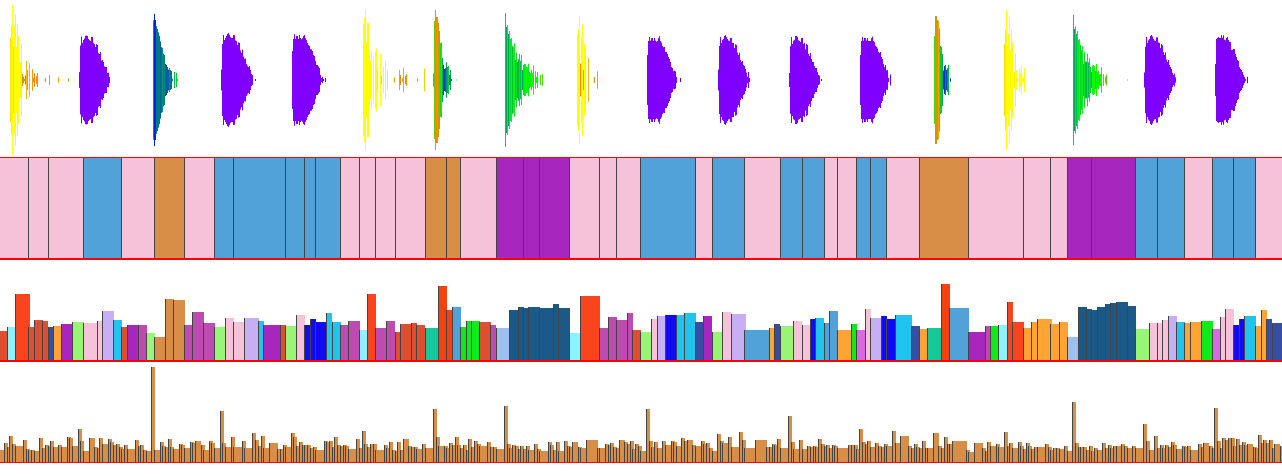
\includegraphics[width=.9\textwidth]{alc_sample}  
\end{center}
\end{frame}

\begin{frame}{Approches Casa \fg algorithmiques \og}
\begin{itemize}
\item Expression d'\textit{a priori} sous forme d'heuristiques computationnelles
\item Algorithmes de structuration non supervisés
\end{itemize}
\begin{block}{Bilan}
\begin{itemize}
\item[\textbf{+}] approches long terme : exploitation d'intervalles d'observation long
\item[\alert{\textbf{-}}] représentation court terme : multi-résolution
\item[\textbf{+}] pas d'apprentissage : protocole expérimental simple, interprétabilité
\item[\alert{\textbf{-}}] pas d'apprentissage : tractabilité, efficience
\end{itemize}
\end{block}
\end{frame}